%===============================================================================
% LaTeX sjabloon voor de bachelorproef toegepaste informatica aan HOGENT
% Meer info op https://github.com/HoGentTIN/latex-hogent-report
%===============================================================================

\documentclass[english,dit,thesis]{hogentreport}

% TODO:
% - If necessary, replace the option `dit`' with your own department!
%   Valid entries are dbo, dbt, dgz, dit, dlo, dog, dsa, soa
% - If you write your thesis in English (remark: only possible after getting
%   explicit approval!), remove the option "dutch," or replace with "english".
\usepackage{xcolor}
\usepackage{listings}
\usepackage{caption} % For proper captions
\usepackage{float} % For H placement specifier
\usepackage{mdframed} % For controlling frames
\usepackage{lipsum} % For blind text, can be removed after adding actual content
\usepackage{placeins}
\usepackage{pifont}                % brings in \ding{}
\usepackage{array}            % for m{width} column
\newcommand{\cmark}{\textcolor{ForestGreen}{\ding{51}}}

% Custom colors for VS Code dark theme
\definecolor{vscodeBackground}{RGB}{30, 30, 30}
\definecolor{vscodeComment}{RGB}{106, 153, 85}
\definecolor{vscodeKeyword}{RGB}{86, 156, 214}
\definecolor{vscodeString}{RGB}{206, 145, 120}
\definecolor{vscodeType}{RGB}{78, 201, 176}
\definecolor{vscodeForeground}{RGB}{220, 220, 220}

% Configure listings for TypeScript code
\lstdefinelanguage{TypeScript}{
  keywords={break, case, catch, continue, debugger, default, delete, do, else, finally, for, function, if, in, instanceof, new, return, switch, this, throw, try, typeof, var, void, while, with, const, let, async, await, class, export, extends, import, super, interface, from},
  keywordstyle=\color{vscodeKeyword},
  ndkeywords={true, false, null, undefined, string, number, boolean, any, void},
  ndkeywordstyle=\color{vscodeType},
  identifierstyle=\color{vscodeForeground},
  sensitive=true,
  comment=[l]{//},
  morecomment=[s]{/*}{*/},
  commentstyle=\color{vscodeComment},
  stringstyle=\color{vscodeString},
  morestring=[b]',
  morestring=[b]"
}

% Define a completely borderless style for code listings
\definecolor{numberGray}{RGB}{100, 100, 100}
\definecolor{lineNumberBg}{RGB}{40, 40, 40}

% Configure main listing style
\definecolor{frameColor}{RGB}{40, 40, 40}

\lstset{
  backgroundcolor=\color{vscodeBackground},
  basicstyle=\small\ttfamily\color{vscodeForeground},
  frame=none,
  framerule=0pt,
  framesep=0pt,
  xleftmargin=15pt,
  xrightmargin=5pt,
  breaklines=true,
  breakatwhitespace=false,
  postbreak=\raisebox{0ex}[0ex][0ex]{\ensuremath{\hookrightarrow\space}},
  tabsize=2,
  numbers=left,
  numberstyle=\tiny\color{numberGray},
  numbersep=10pt,
  showspaces=false,
  showstringspaces=false,
  showtabs=false,
  captionpos=b,
  columns=flexible,
  keepspaces=true,
  aboveskip=1em,
  belowskip=1em
}

% Just use the existing listings setup without trying to redefine environments
\captionsetup[lstlisting]{labelsep=period, labelfont={bf,color=vscodeForeground}, textfont={it,color=vscodeForeground}}

% Create a completely borderless frame for listings
\surroundwithmdframed[hidealllines=true, backgroundcolor=vscodeBackground, innerleftmargin=15pt, innerrightmargin=5pt, skipabove=1em, skipbelow=1em]{lstlisting}

% Add a bit of spacing around listings
\lstset{
  aboveskip=1em,
  belowskip=1em
}
% No need to include enumitem package as it's already loaded in hogentreport.cls
% Enable inline lists feature directly after the document class
\makeatletter
\AtBeginDocument{%
  \@ifpackageloaded{enumitem}{%
    \SetEnumitemKey{inline}{itemjoin={,\ },after=.}%
    \newlist{enumerate*}{enumerate*}{3}%
    \setlist[enumerate*]{label=\arabic*.}%
  }{}%
}

%% Pictures to include in the text can be put in the graphics/ folder
\graphicspath{{../graphics/}}

%% For source code highlighting, requires pygments to be installed
%% Compile with the -shell-escape flag!
\usepackage[chapter]{minted}
%% If you compile with the make_thesis.{bat,sh} script, use the following
%% import instead:
% \usepackage[chapter,outputdir=../output]{minted}
\usemintedstyle{solarized-light}

%% Formatting for minted environments.
\setminted{%
    autogobble,
    frame=lines,
    breaklines,
    linenos,
    tabsize=4
}

%% Ensure listings appear in the list of listings
\renewcommand\listoflistingscaption{%
    \IfLanguageName{dutch}{Lijst van codefragmenten}{List of listings}
}
\renewcommand\listingscaption{%
    \IfLanguageName{dutch}{Codefragment}{Listing}
}
% Make sure the listings package uses our caption/label settings
\let\lst@caption\relax
% Just use the standard listings package command
\renewcommand*\listoflistings{%
    \cleardoublepage\phantomsection\addcontentsline{toc}{chapter}{\listoflistingscaption}%
    \lstlistoflistings%
}

% Other packages not already included can be imported here

%%---------- Document metadata -------------------------------------------------
% TODO: Replace this with your own information
\author{Abdellah El Halimi}
\supervisor{Dhr. A. De Witte}
\cosupervisor{Dhr. C. Dutoict}
% \title[Optionele ondertitel]%
%     {Titel van de bachelorproef}
\title{Accessible Password Management Using Face Recognition for Individuals with Cognitive and Motor Disabilities}
\academicyear{2024-2025}
\examperiod{1}
\degreesought{\IfLanguageName{dutch}{Professionele bachelor in de toegepaste informatica}{Bachelor of applied computer science}}
\partialthesis{false} %% To display 'in partial fulfilment'
%\institution{Internshipcompany BVBA.}

%% Add global exceptions to the hyphenation here
\hyphenation{back-slash}

%% The bibliography (style and settings are  found in hogentthesis.cls)
\addbibresource{bachproef.bib}            %% Bibliography file
\addbibresource{../voorstel/voorstel.bib} %% Bibliography research proposal
\defbibheading{bibempty}{}

%% Prevent empty pages for right-handed chapter starts in twoside mode
\renewcommand{\cleardoublepage}{\clearpage}

\renewcommand{\arraystretch}{1.2}

%% Content starts here.
\begin{document}

%---------- Front matter -------------------------------------------------------

\frontmatter

\hypersetup{pageanchor=false} %% Disable page numbering references

%% Render a Dutch outer title page if the main language is English
% \IfLanguageName{english}{%
%     %% If necessary, information can be changed here
%     \degreesought{Professionele Bachelor toegepaste informatica}%
%     \begin{otherlanguage}{dutch}%
%        \maketitle%
%     \end{otherlanguage}%
% }{}

%% Generates title page content
\maketitle
\hypersetup{pageanchor=true}

%%=============================================================================
%% Voorwoord
%%=============================================================================

\chapter*{\IfLanguageName{dutch}{Woord vooraf}{Preface}}%
\label{ch:voorwoord}

%% TODO:
%% Het voorwoord is het enige deel van de bachelorproef waar je vanuit je
%% eigen standpunt (``ik-vorm'') mag schrijven. Je kan hier bv. motiveren
%% waarom jij het onderwerp wil bespreken.
%% Vergeet ook niet te bedanken wie je geholpen/gesteund/... heeft

\lipsum[1-2]
%%=============================================================================
%% Samenvatting
%%=============================================================================

% TODO: De "abstract" of samenvatting is een kernachtige (~ 1 blz. voor een
% thesis) synthese van het document.
%
% Een goede abstract biedt een kernachtig antwoord op volgende vragen:
%
% 1. Waarover gaat de bachelorproef?
% 2. Waarom heb je er over geschreven?
% 3. Hoe heb je het onderzoek uitgevoerd?
% 4. Wat waren de resultaten? Wat blijkt uit je onderzoek?
% 5. Wat betekenen je resultaten? Wat is de relevantie voor het werkveld?
%
% Daarom bestaat een abstract uit volgende componenten:
%
% - inleiding + kaderen thema
% - probleemstelling
% - (centrale) onderzoeksvraag
% - onderzoeksdoelstelling
% - methodologie
% - resultaten (beperk tot de belangrijkste, relevant voor de onderzoeksvraag)
% - conclusies, aanbevelingen, beperkingen
%
% LET OP! Een samenvatting is GEEN voorwoord!

%%---------- Nederlandse samenvatting -----------------------------------------
%
% TODO: Als je je bachelorproef in het Engels schrijft, moet je eerst een
% Nederlandse samenvatting invoegen. Haal daarvoor onderstaande code uit
% commentaar.
% Wie zijn bachelorproef in het Nederlands schrijft, kan dit negeren, de inhoud
% wordt niet in het document ingevoegd.

\IfLanguageName{english}{%
\selectlanguage{dutch}
\chapter*{Samenvatting}
De toenemende afhankelijkheid van online diensten heeft het belang van wachtwoordbeheer in digitale beveiliging versterkt. Traditionele authenticatiemethoden, zoals het invoeren en onthouden van complexe wachtwoorden, vormen vaak aanzienlijke uitdagingen voor personen met cognitieve of motorische beperkingen, waaronder moeilijkheden met geheugen of manuele input. Deze beperkingen onderstrepen de dringende nood aan toegankelijke authenticatieoplossingen die zowel de gebruiksvriendelijkheid als de tevredenheid van de gebruiker verbeteren.

De centrale onderzoeksvraag luidt: \emph{Hoe kan gezichtsherkenningstechnologie de toegankelijkheid van wachtwoordbeheer verbeteren voor personen met cognitieve en motorische beperkingen?}

Het doel van deze bachelorproef is het ontwerpen van een wachtwoordmanager op basis van gezichtsherkenning, specifiek gericht op personen met cognitieve of motorische beperkingen.

Het onderzoek omvat een vergelijkende analyse van verschillende gezichtsherkennings-API’s in diverse programmeertalen om de meest geschikte technologiestack te bepalen. Met de geselecteerde tools werd vervolgens een webgebaseerd prototype van een wachtwoordmanager ontwikkeld. Het prototype volgt een hybride architectuur waarbij de browser verantwoordelijk is voor gezichtsdetectie en client-side versleuteling van de beelden, terwijl de server instaat voor het extraheren van gezichtskenmerken, het uitvoeren van vergelijkingen en het veilig opslaan van de gegevens.

Indien het prototype veelbelovende resultaten oplevert, zal in een vervolgfase een browserextensie ontwikkeld worden om de schaalbaarheid en doeltreffendheid van de gekozen oplossingen in een realistische gebruiksomgeving te evalueren. Deze iteratieve aanpak maakt een gestructureerde evaluatie van de technologieën mogelijk vóór volledige implementatie.

De verwachte resultaten omvatten een verbeterde toegankelijkheid en gebruiksgemak ten opzichte van traditionele wachtwoordbeheerders, wat leidt tot een hogere gebruikerstevredenheid en minder frustratie tijdens het inloggen. Deze studie beoogt het potentieel van gezichtsherkenning aan te tonen om reële toegankelijkheidsproblemen in digitaal identiteitsbeheer aan te pakken, en zo personen met een beperking in staat te stellen hun inloggegevens zelfstandig en veilig te beheren.
\selectlanguage{english}
}{}

%%---------- Samenvatting -----------------------------------------------------
% De samenvatting in de hoofdtaal van het document

\chapter*{\IfLanguageName{dutch}{Samenvatting}{Abstract}}

The increasing reliance on online services has elevated the importance of password management in digital security. Traditional authentication methods, such as typing and remembering complex passwords, often pose significant challenges for individuals with cognitive or motor disabilities, including difficulties with memory recall or manual input. These limitations highlight the urgent need for accessible authentication solutions that improve both user satisfaction and usability.

The central research question is: \emph{How can face recognition technology improve accessibility in password management for individuals with cognitive and motor disabilities?} 

The objective of this thesis is to design a facial recognition-based password manager specifically aimed at individuals with cognitive or motor impairments.

The research includes a comparative analysis of several facial-recognition APIs across multiple programming languages to determine the best technology stack, and a web-based prototype password manager was then built with the selected tools. The prototype follows a hybrid architecture in which the browser executes face detection and client-side encryption of captured images, while the server performs descriptor extraction, matching, and secure storage.

If the prototype yields promising results, a browser extension will be developed as a follow-up to evaluate the scalability and effectiveness of the selected solutions in a realistic use context. This iterative approach enables a structured evaluation of technologies prior to full implementation.

The anticipated outcomes include improved accessibility and ease of use compared to traditional password managers, leading to increased user satisfaction and reduced frustration during authentication. This study aims to demonstrate the potential of facial recognition to address real-world accessibility barriers in digital identity management, thereby empowering users with disabilities to manage their credentials independently and securely.


%---------- Inhoud, lijst figuren, ... -----------------------------------------

\tableofcontents

% In a list of figures, the complete caption will be included. To prevent this,
% ALWAYS add a short description in the caption!
%
%  \caption[short description]{elaborate description}
%
% If you do, only the short description will be used in the list of figures

% \listoffigures  % Commented out - no figures in thesis

% If you included tables and/or source code listings, uncomment the appropriate
% lines.
\listoftables

\listoflistings

% Als je een lijst van afkortingen of termen wil toevoegen, dan hoort die
% hier thuis. Gebruik bijvoorbeeld de ``glossaries'' package.
% https://www.overleaf.com/learn/latex/Glossaries

%---------- Kern ---------------------------------------------------------------

\mainmatter{}

% De eerste hoofdstukken van een bachelorproef zijn meestal een inleiding op
% het onderwerp, literatuurstudie en verantwoording methodologie.
% Aarzel niet om een meer beschrijvende titel aan deze hoofdstukken te geven of
% om bijvoorbeeld de inleiding en/of stand van zaken over meerdere hoofdstukken
% te verspreiden!

%%=============================================================================
%% Inleiding
%%=============================================================================

\chapter{\IfLanguageName{dutch}{Inleiding}{Introduction}}%
\label{ch:inleiding}

In today's digital age, authentication is a crucial element of cybersecurity. Traditional password-based systems require users to create, remember, and accurately enter complex passwords. For individuals with cognitive or motor disabilities, this process presents significant challenges that can lead to frustration, frequent lockouts, and increased security risks. This thesis investigates the integration of face recognition technology into a password manager to develop an accessible and user-friendly authentication method.

\subsection{Context and Background}
The increasing reliance on online services has amplified the need for secure and accessible authentication solutions. Conventional methods, such as passwords, often fail to accommodate the unique needs of users with disabilities. Cognitive impairments may hinder memory recall, while motor disabilities can complicate the physical act of typing. These challenges underscore the necessity for an alternative approach—one that minimizes cognitive and physical burdens without compromising security. In this context, the proposed research explores the use of face recognition technology as a viable solution to enhance digital authentication.

\subsection{Justification of the Topic}
This research focuses exclusively on evaluating face recognition as an alternative to traditional master passwords in a web-based password manager. Key points include:
\begin{itemize}
  \item \textbf{Target Group:} Individuals with cognitive and motor disabilities.
  \item \textbf{Tool Selection:} Emphasis on tools like \texttt{face-api.js}, which operate entirely in the browser to ensure privacy by eliminating server-side processing.
  \item \textbf{Alignment:} Integration with modern web technologies and adherence to accessibility standards.
\end{itemize}

\section{\IfLanguageName{dutch}{Probleemstelling}{Problem Statement}}%
\label{sec:probleemstelling}

Traditional password systems impose substantial cognitive and physical demands on users, particularly those with disabilities. The inherent complexity of creating, remembering, and entering passwords can significantly reduce user autonomy and lead to security vulnerabilities. This research seeks to determine how face recognition technology can replace traditional passwords in a way that overcomes these challenges—ultimately providing a more accessible and secure solution for the target group.

\section{\IfLanguageName{dutch}{Onderzoeksvraag}{Research Question}}%
\label{sec:onderzoeksvraag}

The central research question of this thesis is:
\begin{quote}
How can face recognition technology be effectively integrated into a password manager to improve accessibility for individuals with cognitive and motor disabilities?
\end{quote}

To explore this question further, the following sub-questions will be addressed:
\begin{enumerate}
  \item What specific challenges do individuals with cognitive and motor disabilities face with traditional password systems?
  \item How does face recognition technology compare to conventional methods in terms of usability and security?
  \item What are the technical requirements and potential obstacles for incorporating face recognition into existing password management systems?
\end{enumerate}

\section{\IfLanguageName{dutch}{Onderzoeksdoelstelling}{Research Objective}}%
\label{sec:onderzoeksdoelstelling}

The primary objective of this thesis is to design and develop a proof-of-concept web-based password manager that utilizes face recognition for user authentication. Success will be measured against the following criteria:
\begin{itemize}
  \item \textbf{Enhanced Accessibility:} Reducing the cognitive and physical effort required during authentication.
  \item \textbf{Improved Security:} Addressing vulnerabilities inherent in text-based passwords.
  \item \textbf{User-Friendly Interface:} Adhering to Web Content Accessibility Guidelines (WCAG) to ensure ease of use for the target audience.
\end{itemize}

\section{\IfLanguageName{dutch}{Opzet van deze bachelorproef}{Structure of this Bachelor Thesis}}%
\label{sec:opzet-bachelorproef}

% Het is gebruikelijk aan het einde van de inleiding een overzicht te
% geven van de opbouw van de rest van de tekst. Deze sectie bevat al een aanzet
% die je kan aanvullen/aanpassen in functie van je eigen tekst.

De rest van deze bachelorproef is als volgt opgebouwd:

In Hoofdstuk~\ref{ch:stand-van-zaken} wordt een overzicht gegeven van de stand van zaken binnen het onderzoeksdomein, op basis van een literatuurstudie.

In Hoofdstuk~\ref{ch:methodologie} wordt de methodologie toegelicht en worden de gebruikte onderzoekstechnieken besproken om een antwoord te kunnen formuleren op de onderzoeksvragen.

% TODO: Vul hier aan voor je eigen hoofstukken, één of twee zinnen per hoofdstuk

In Hoofdstuk~\ref{ch:conclusie}, tenslotte, wordt de conclusie gegeven en een antwoord geformuleerd op de onderzoeksvragen. Daarbij wordt ook een aanzet gegeven voor toekomstig onderzoek binnen dit domein.
\chapter{\IfLanguageName{dutch}{Stand van zaken}{State of the art}}%
\label{ch:stand-van-zaken}

% Tip: Begin elk hoofdstuk met een paragraaf inleiding die beschrijft hoe
% dit hoofdstuk past binnen het geheel van de bachelorproef. Geef in het
% bijzonder aan wat de link is met het vorige en volgende hoofdstuk.

% Pas na deze inleidende paragraaf komt de eerste sectiehoofding.


% TODO: GDPR regulations about storing face data/imgs

\section{Authentication in Digital Security}
Authentication is the process of verifying the identity of users attempting to access digital systems or online services. 
Commonly used methods include knowledge-based authentication (passwords), possession-based methods (tokens), and 
biometric methods like fingerprints and facial recognition \autocite{Pant2022}. Passwords remain dominant due to 
their simplicity and widespread acceptance, but face security issues including password reuse, phishing, and 
brute-force attacks \autocite{Ophoff2021}. For users with cognitive or motor disabilities, these issues are 
further complicated by difficulties in recalling or accurately inputting passwords \autocite{Rochford2014}.

\section{Accessibility Challenges in Authentication}
Individuals with cognitive disabilities, such as memory disorders or conditions like dyslexia, often struggle with remembering complex passwords, resulting in frequent authentication failures and frustration \autocite{Farid2019, Ophoff2021}. Those with motor disabilities, including conditions like Parkinson's disease or cerebral palsy, face physical challenges in typing passwords accurately \autocite{Renaud2020}. The Web Content Accessibility Guidelines (WCAG) highlight the importance of designing authentication systems that minimize these cognitive and physical burdens \autocite{Brewer2023}.

\vspace{4\baselineskip}
\section{Facial Recognition Technology}
Facial recognition works by identifying and verifying individuals from digital images or videos using various algorithmic approaches, including traditional image processing methods and modern deep learning techniques. Notable algorithms include Haar cascades, Eigenfaces, Local Binary Patterns Histograms (LBPH), and Convolutional Neural Networks (CNNs) \autocite{ElSayed2015}. The evolution of deep learning, particularly CNN-based approaches, has significantly enhanced accuracy and reliability, making facial recognition robust even under challenging conditions like variations in lighting, angle, or facial expressions \autocite{ZhangDlib2020}.

\section{Face Recognition as a Biometric Solution}
Biometric authentication, particularly facial recognition, is gaining popularity as it significantly reduces the cognitive and physical effort required by traditional password-based methods \autocite{Furnell2022}. 
Unlike passwords, biometric data are unique physical attributes of an individual, providing an inherent security advantage by eliminating risks associated with knowledge-based authentication methods, 
such as forgetting or sharing passwords \autocite{Pant2022}.

Facial recognition stands out as particularly promising because it is intuitive, does not require manual dexterity, and can be seamlessly integrated into daily digital interactions \autocite{Bhatt2011}. However, biometric systems are not without limitations. Spoofing attacks, privacy concerns, and the requirement for consistent lighting and camera quality present technical and ethical considerations that must be carefully managed \autocite{Kuznetsov2024, Bahia2024}.


\subsection{Comparison of Facial Recognition Libraries}

\subsubsection{OpenCV (Java)}
OpenCV is a widely used open-source library offering classical computer vision techniques such as Haar cascades and LBPH. While effective in controlled environments, it typically requires server-side or desktop-based implementations, limiting its applicability for client-side web applications \autocite{Dominguez2017}.

\subsubsection{face\_recognition in Python}  
The face\_recognition library, built on dlib, is renowned for its accuracy and pre-trained deep learning models. \textcite{ZhangDlib2020} highlight that it excels in applications requiring precision, utilizing techniques like CNN-based face encodings for high-quality results. However, its reliance on Python and backend processing makes it less suitable for client-side, browser-based implementations like those required in this project.

\subsubsection{face-api.js (JavaScript)}
face-api.js, built on TensorFlow.js, runs entirely in the browser, providing a privacy-centric, client-side solution suitable for real-time applications \autocite{Vageele2024}. Its key benefits include privacy (no server-side data transfer), compatibility with modern web frameworks, and modularity for lightweight and efficient real-time processing. These features align closely with the project's emphasis on usability, accessibility, and security, making face-api.js the optimal choice for this research.

\section{Security Considerations for Biometric Authentication}
While facial recognition enhances accessibility, it also introduces specific security concerns. Common vulnerabilities include spoofing attacks using photos or video recordings and data privacy issues related to biometric data storage \autocite{Bowyer2006, Bahia2024}. Beyond these well-known threats, systems that store facial biometric data face additional sophisticated attack vectors:

\begin{itemize}
\item \textbf{Template Extraction Attacks:} These attacks aim to reconstruct biometric templates from stored embeddings, potentially compromising the entire authentication system. Even when templates are encrypted, side-channel attacks can leak information about the underlying biometric data \autocite{Mai2019, Dong2021}. As demonstrated by \textcite{Mai2019}, deep face templates previously thought to be secure can be reverse-engineered to recover recognizable face images, raising significant privacy concerns. Building on this work, \textcite{Dong2021} showed that high-definition face images can be generated from supposedly secure templates using advanced generative models.

\item \textbf{Model Inversion Attacks:} Adversaries can exploit machine learning models to regenerate facial images from stored embeddings or model parameters, effectively reversing the feature extraction process \autocite{Fredrikson2015, Zhang2020}. \textcite{Fredrikson2015} demonstrated that these attacks can leverage confidence information from ML models to reconstruct training data, while \textcite{Zhang2020} advanced this concept with generative model-inversion attacks against deep neural networks. This poses significant privacy risks as it may allow attackers to recreate recognizable facial images from supposedly secure numerical representations.

\item \textbf{Spoofing Attacks:} Presentation attacks using photos or video recordings of legitimate users to deceive recognition systems \autocite{Kuznetsov2024}.
\end{itemize}

Modern mitigation strategies include:
\begin{itemize}
\item \textbf{Liveness Detection:} Techniques to ensure the presence of a real, live user rather than a static image or video \autocite{Kuznetsov2024}.

\item \textbf{Local Data Processing:} Client-side processing prevents the transmission of sensitive biometric data, enhancing privacy.

\item \textbf{Multi-factor Authentication (MFA):} Combining biometric data with other authentication methods to provide layers of security and protect against vulnerabilities inherent in single-method authentication systems \autocite{Furnell2022}.

\item \textbf{Cancelable Biometrics:} Applying irreversible transformations to biometric templates before storage, allowing for template revocation if compromised. \textcite{Rathgeb2011} provide a comprehensive survey of these techniques, highlighting their importance in protecting biometric data while maintaining authentication accuracy.
\end{itemize}

\section{Adversary Threat Models in Facial Biometric Authentication}
Modern facial biometric systems must account for various adversary capabilities and attack vectors. Table 1 summarizes three critical threats and effective mitigation strategies, with references to recent literature and technical reports.

\begin{table}[htbp]
  \centering
  \small
  \begin{tabular}{|p{3.2cm}|p{6.2cm}|p{5.8cm}|}
    \hline
    \textbf{Threat} & \textbf{Description} & \textbf{Mitigation(s)} \\
    \hline
    \textbf{Offline Database Theft} & Adversary gains unauthorized access to stored biometric templates or face embeddings (e.g., via a database breach). Stolen biometric data can be misused for identity theft or cross-system fraud, since compromised templates allow attackers to impersonate users or perform cross-matching across different services. (Unlike passwords, biometric traits are permanent, so a leaked template poses a long-term risk to the victim.) & Protect stored templates using strong cryptography and transform-based protections. Encrypt biometric databases at rest so stolen files are unusable, and apply non-invertible, revocable transformations (i.e. **cancelable biometrics**) to the templates. Cancelable biometric schemes store only a transformed version of the face data that cannot be reversed and can be *“revoked”* or replaced if compromised. Additional safeguards include multi-factor authentication - ensuring a biometric alone cannot unlock accounts - and hardware security modules for template storage, which together limit the damage from a stolen biometric database. \\
    \hline
    \textbf{Compromised Browser Extension} & A malicious or compromised browser extension (or similar client-side malware) intercepts facial data during capture or transmission. The attacker could tap into the live camera feed or extracted face embeddings and steal or manipulate this data in real time. This essentially creates a man-in-the-middle, allowing replay or injection of captured biometric data to fraudulently authenticate as the victim. *In fact, recent banking malware has been observed recording victims' faces and using AI-generated videos (deepfakes) to bypass facial authentication defenses.* & Isolate and secure the biometric processing on the client side, minimizing the extension's access to sensitive data. For example, perform face recognition in a trusted local environment (using in-browser ML libraries or OS-level APIs) so that raw images/embeddings aren't sent over the network. All communication between the browser and any authentication server should be encrypted end-to-end, preventing eavesdropping or tampering in transit. It's also wise to require explicit user presence or a secondary factor (MFA) before finalizing login. This way, even if an extension is compromised, an attacker cannot stealthily authenticate with stolen biometrics alone. Robust code signing and permission controls on extensions further reduce the risk of compromise. \\
    \hline
    \textbf{Shoulder-Surfing} & An attacker observes or records the legitimate user's face during an authentication attempt (e.g., looking over the user's shoulder or using a camera from nearby). By capturing the user's facial input, the adversary can later present a **spoof** - such as a photo, video, or mask of the user's face - to impersonate them. Biometric systems eliminate the need to type passwords (mitigating classic shoulder-surfing of secrets), but without countermeasures they remain vulnerable to replay attacks using captured biometric data. In essence, a clear image or video of the user can be “replayed” to fool a naïve face recognition system. & Deploy anti-spoofing and liveness detection measures to ensure the system is interacting with a live user *in real time* rather than a recording or static image. Effective liveness detection techniques include prompting the user to perform random actions (e.g. blink, turn head) or using 3D/infrared cameras to detect depth and vitality cues, which defeats simple photo or video replays. Advanced deep-learning-based **face anti-spoofing** can automatically classify and reject fake vs. live imagery. Furthermore, requiring user attention or a secondary confirmation (such as a phone notification or a known gesture) can mitigate the risk of covert observation. By combining these defenses - liveness verification and optional multi-factor checks - facial authentication systems become much more resistant to shoulder-surfing and presentation attacks. \\
    \hline
  \end{tabular}
  \caption{Adversary capabilities and example mitigations for facial biometric authentication systems.}
  \label{tab:threat-model}
\end{table}


\section{Current Limitations in Password Managers}
Password managers simplify password management by securely storing and auto-filling credentials but commonly rely on a master password, perpetuating cognitive and motor accessibility issues. This approach is problematic for users who struggle with memory recall or precise typing \autocite{IALabs2024}. While MFA offers increased security, it often introduces additional complexity that further burdens users with disabilities. Current systems have limited inclusivity and accessibility, reinforcing the need for more intuitive solutions.

\section{Database Options for Client\textendash Side Password Storage}
\label{sec:db-options}

A password manager must choose a local datastore that balances footprint,
offline capability, security, and future synchronisation needs.  The five
candidates below are summarised with literature references and official
documentation links; each paragraph is kept within seven lines for brevity.

\subsection*{SQLite}
\textcite{Gaffney2022} show that SQLite embeds the entire ACID-compliant
engine in a single file of only a few-hundred-kB, requiring no server
process.  Its dynamic typing allows flexible schemas \autocite{Corovcak2025}.
Because it lacks native user authentication, security depends on OS file
permissions or extensions such as SQLCipher \autocite{Corovcak2025}.
Official documentation confirms the zero-config model and SQL feature set
\autocite{sqlLiteDoc2025}.  These traits make SQLite ideal for an offline,
single-device password vault, provided the file is encrypted at rest.

\subsection*{PostgreSQL}
PostgreSQL's client-server design provides robust concurrency and rich SQL
features after 35-years of development \autocite{Gkamas2022}.  It supports
role-based access control and TLS for data in transit, yet the community
edition offers no built-in at-rest encryption—administrators must use
\textit{pgcrypto} or file-system measures \autocite{Crunchy2024,
PostgreSQL2025}.  A local instance typically consumes hundreds of-MB of RAM,
which is heavy for a mobile vault.  Hence PostgreSQL is secure and scalable,
but over-provisioned for a single-user client.

\subsection*{MongoDB}
MongoDB stores JSON-like documents in flexible collections and scales
horizontally \autocite{Miryala2024}.  A \texttt{mongod} process needs 1-2-GB
RAM even for modest use \autocite{Dahunsi2021}.  Community builds provide
authentication and TLS, yet encryption at rest is Enterprise-only
\autocite{PrismaMongoEnc, MongoDB2025}, so disk encryption or field-level
crypto is required.  Misconfiguration has repeatedly exposed databases,
underscoring the need for hardened defaults \autocite{SqlLite2025}.  The
server footprint makes MongoDB ill-suited to a purely offline desktop
password manager.

\subsection*{Couchbase Lite}
Couchbase Lite embeds a document store inside the app and syncs through
Sync Gateway when online \autocite{Pal2016}.  Its metadata inflates on-disk
size versus SQLite, yet runtime demands remain mobile-friendly
\autocite{Gkamas2022}.  The Enterprise build supports 256-bit AES encryption
of the local DB \autocite{CouchbaseEncryption, CouchbaseDoc2025}.  Because it
executes in the app's sandbox, further authentication is handled by the host
application.  These qualities make Couchbase Lite attractive for an
offline-first vault that may later sync across devices.

\subsection*{Firebase Cloud Firestore}
Firestore is a serverless NoSQL service that caches data locally and
synchronises transparently once connectivity returns \autocite{FirebaseDoc2025}.
Security combines Firebase Authentication with declarative Firestore Rules,
while Google encrypts data in transit and at rest \autocite{FirebaseSecurity2025}.
This offloads database maintenance but requires Internet access for initial
login and long-term storage.  Firestore therefore suits a multi-device,
cloud-centric password manager but cedes full data custody to Google.


\section{Cryptographic Security in Password Managers}
Secure storage of credentials is fundamental in password management.  
In this project, every cryptographic operation executes client-side with the
\texttt{crypto-js} library \autocite{CryptoJS2024}, combining AES-256 for
confidentiality and PBKDF2 for key derivation.  AES supplies a
NIST-approved block cipher \autocite{NISTFIPS197}, while PBKDF2's 10\,000
iterations and per-installation salt greatly raise the cost of brute-force
attacks \autocite{RFC8018}.  Keeping both encryption and decryption in the
browser ensures plaintext credentials or biometric images never leave the
device, aligning with OWASP key-management guidance
\textcite{OWASPKeyMgmt2025}.

\subsubsection{Crypto-js}  
The \texttt{crypto-js} library offers JavaScript implementations of AES,
PBKDF2, and other standard algorithms through a concise API optimised for the
browser.  Its widespread adoption and open-source governance mean the code
base is continuously scrutinised and updated for vulnerabilities
\autocite{CryptoJS2024}.

\subsubsection{AES}  
AES-256 encrypts both passwords and face images, providing a large key space
and proven resistance to cryptanalysis.  Defined in FIPS 197, AES remains the
de-facto standard for protecting electronic data across government and
industry \autocite{NISTFIPS197}. 

\subsubsection{Encryption Key Handling}  
Each encryption key is derived in the browser at login and kept only in
memory; it is never persisted or sent to the backend.  This client-centric
approach follows OWASP key-management recommendations, ensuring a server
breach alone cannot expose decryption keys
\autocite{OWASPKeyMgmt2025}. 

\subsubsection{PBKDF2}  
PBKDF2, specified in RFC 8018, transforms the user's secret into a strong
256-bit key using 10\,000 iterations and a unique 16-byte salt.  Iterative
key stretching slows dictionary attacks, while the salt thwarts rainbow
tables \autocite{RFC8018}.

\section{Usability and Accessibility Standards}
Accessibility in digital solutions adheres to guidelines such as WCAG, which outline best practices for minimizing cognitive load, ensuring interface clarity, and reducing physical input requirements. Adopting these standards ensures the password manager prototype remains usable for individuals with various disabilities \autocite{Brewer2023}. Inclusive design principles further emphasize the need to involve users with disabilities in the development process to validate and refine usability \autocite{Lazar2015}.

\subsection{WCAG 2.1 Compliance Framework}
A comprehensive approach to accessibility requires systematic mapping of features against established standards. The table below provides a traceability matrix that maps the password manager's features to the Web Content Accessibility Guidelines (WCAG 2.1) success criteria. This matrix serves as both a design reference and a verification tool to ensure all accessibility requirements are addressed in the implementation phase. When we discuss the usability study design in Chapter~\ref{ch:methodologie}, we will reference this matrix to highlight which criteria were empirically verified through user testing.

\begin{table}[htbp]
  \centering
  \small
  \begin{tabular}{|p{2.5cm}|p{1.5cm}|p{4cm}|p{4cm}|p{1.2cm}|}
    \hline
    \textbf{WCAG 2.1} & \textbf{Con-} & \textbf{Features} & \textbf{Evidence / Implementation} & \textbf{Status} \\
    \textbf{Success} & \textbf{formance} & & & \\
    \textbf{Criterion} & \textbf{Level} & & & \\ \hline
    
    1.1.1 Non-text Content & A & Face-registration and authentication UI, credential icons, action buttons & alt text for static images; ARIA labels (e.g. aria-label="Capture selfie") on camera controls & Pass \\ \hline
    
    1.3.1 Info \& Relationships & A & Modal forms for Add / Edit Credential, list view of saved credentials & Implemented with semantic HTML elements (\texttt{<form>}, \texttt{<label>}, \texttt{<ul>/<li>}); programmatic labels bound to inputs & Pass \\ \hline
    
    1.3.2 Meaningful Sequence & A & React component hierarchy for registration \& login flows & DOM order matches visual order; logical tab order verified with keyboard & Pass \\ \hline
    
    1.3.4 Orientation & AA & Responsive layout (CSS Flex/Grid) & UI adapts to both portrait and landscape on mobile; no fixed-orientation lock & Pass \\ \hline
    
    1.4.3 Contrast (Minimum) & AA & Global Tailwind theme & Colour palette tested with WCAG contrast checker: all text/background combinations $\geq$ 4.5:1 & Pass \\ \hline
    
    1.4.5 Images of Text & AA & Credential list, buttons & No UI element relies on rasterised text; all labels are true text & Pass \\ \hline
    
    1.4.10 Reflow & AA & Responsive UI on small screens & Tested to 320 px width without horizontal scroll & Pass \\ \hline
    
    1.4.11 Non-text Contrast & AA & Icon buttons, focus rings & SVG icons meet 3:1 contrast; focus outline uses high-contrast colour & Pass \\ \hline
    
    2.1.1 Keyboard & A & All interactive controls & tabIndex flows through modals and lists; face-capture can be triggered with Enter key & Pass \\ \hline
    
    2.1.2 No Keyboard Trap & A & Modal dialogs & Esc, Tab and Shift+Tab correctly move focus or close modal & Pass \\ \hline
  \end{tabular}
  \caption[WCAG 2.1 Traceability Matrix]{WCAG 2.1 Traceability Matrix for the Face-Based Password Manager. This matrix maps features of the prototype to relevant Web Content Accessibility Guidelines success criteria, demonstrating how the design addresses accessibility requirements.}
  \label{tab:wcag-matrix}
\end{table}

\begin{table}[htbp]
  \centering
  \small
  \begin{tabular}{|p{2.5cm}|p{1.5cm}|p{4cm}|p{4cm}|p{1.2cm}|}
    \hline
    \textbf{WCAG 2.1} & \textbf{Con-} & \textbf{Features} & \textbf{Evidence / Implementation} & \textbf{Status} \\
    \textbf{Success} & \textbf{formance} & & & \\
    \textbf{Criterion} & \textbf{Level} & & & \\ \hline
    
    2.2.1 Timing Adjustable & A & Face-capture countdown & 5-second default, user can extend to 15 s via settings & Pass \\ \hline
    
    2.3.1 Three Flashes or Below & A & Toast animations & All animations < 3 flashes/sec; none are bright flashes & Pass \\ \hline
    
    2.4.3 Focus Order & A & Credential list, modals & Logical sequential focus verified with screen-reader & Pass \\ \hline
    
    2.4.4 Link Purpose & A & External links in footer/help & Link text describes destination (e.g. "WCAG Quick-Ref") & Pass \\ \hline
    
    2.4.7 Focus Visible & AA & Custom focus outline & Uses 2 px outline + 4 px offset to meet visibility & Pass \\ \hline
    
    3.2.1 On Focus & A & Input fields, buttons & No unexpected context changes on focus & Pass \\ \hline
    
    3.2.2 On Input & A & Credential forms & Only explicit Save triggers state change; live form validation announced politely & Pass \\ \hline
    
    3.3.1 Error Identification & A & Form validation & Error messages displayed inline and exposed via aria-describedby & Pass \\ \hline
    
    3.3.2 Labels or Instructions & A & All form inputs, face-capture & Clear labels ("Email Address") and helper text ("Look straight at the camera") & Pass \\ \hline
    
    4.1.1 Parsing & A & React front-end templates & JSX compiles to valid HTML; no duplicate IDs & Pass \\ \hline
    
    4.1.2 Name, Role, Value & A & Custom components (Modal, Button, Toast) & Roles and states exposed with ARIA (role="dialog", aria-modal="true", aria-live="polite") & Pass \\ \hline
  \end{tabular}
  \caption[WCAG 2.1 Traceability Matrix (continued)]{WCAG 2.1 Traceability Matrix for the Face-Based Password Manager (continued).}
  \label{tab:wcag-matrix-cont}
\end{table}

\section{Research-Based Accuracy Benchmarks for Facial Recognition}

In addition to usability, it is important to evaluate the security accuracy of the facial authentication. While a full-scale laboratory test of false acceptance and rejection rates is beyond the scope of our small-sample usability study, we can approximate expectations by citing published benchmarks from similar biometric systems. These provide a reference point for how our prototype should perform in terms of False Accept Rate (FAR) and False Reject Rate (FRR).

\textbf{Windows Hello (IR Facial Login):} Microsoft’s Windows Hello face authentication system, which uses infrared imaging, sets stringent hardware requirements with a FAR of less than 0.001\% (i.e., fewer than 1 in 100{,}000 impostor attempts succeed) \autocite{MicrosoftHelloDocs}. In practice, Microsoft reports a FRR under 5\% without liveness detection, and under 10\% when anti-spoofing measures are enabled \autocite{MicrosoftHelloDocs}. While our web-based prototype (using a standard camera and \texttt{face-api.js}) cannot match these hardware-accelerated standards, it aims to follow the same design philosophy: prioritizing a low FAR even at the expense of occasional false rejects.

\textbf{Apple Face ID (3D Face Recognition):} Apple’s Face ID system also uses 3D infrared facial imaging and targets an extremely low FAR, citing less than 1 in 1{,}000{,}000 chances of unauthorized access \autocite{BentoFaceID}. Although Apple has not disclosed detailed FRR statistics, empirical data suggests that its performance remains highly accurate for legitimate users in normal conditions, despite occasional false rejects caused by sunglasses or facial obstructions. As such, high-end consumer systems aim for FAR values between $10^{-5}$ and $10^{-6}$, while keeping FRR below 10\%.

\textbf{Academic Benchmarks (FRVT and Others):} Independent evaluations, such as the U.S. National Institute of Standards and Technology (NIST) Face Recognition Vendor Test (FRVT), provide authoritative insight. A top-performing algorithm in FRVT 1:1 verification achieved a false non-match rate of 0.36\% at a FAR of 1 in 1{,}000{,}000 \autocite{ParavisionFRVT}. These results represent optimal conditions; performance degrades in less-controlled environments such as those encountered by webcam-based authentication. Nonetheless, they indicate the capabilities of modern face recognition technologies.

\textbf{Typical Web/Mobile Authentication:} For systems using standard RGB cameras, face recognition APIs such as Microsoft Azure Face and Amazon Rekognition typically report over 99\% true acceptance rates under good conditions \autocite{IJCAFace}. Benchmarks on datasets like LFW (Labeled Faces in the Wild) indicate that many models achieve 99.5\%+ identification accuracy in uncontrolled photographic conditions. The UK National Cyber Security Centre estimates a FAR better than 0.1\% and FRR between 5--10\% for mobile face unlock systems \autocite{BentoFaceID,MicrosoftHelloDocs}.

Using these references, we propose that our prototype should aim for a FAR in the range of $\leq$0.1\% to prevent unauthorized access, while tolerating a FRR of 5--10\% as a reasonable usability trade-off. We conservatively set the matching threshold in our system to favor security, accepting that users may occasionally need to retry under suboptimal conditions.



% \begin{figure}
%   \centering
%   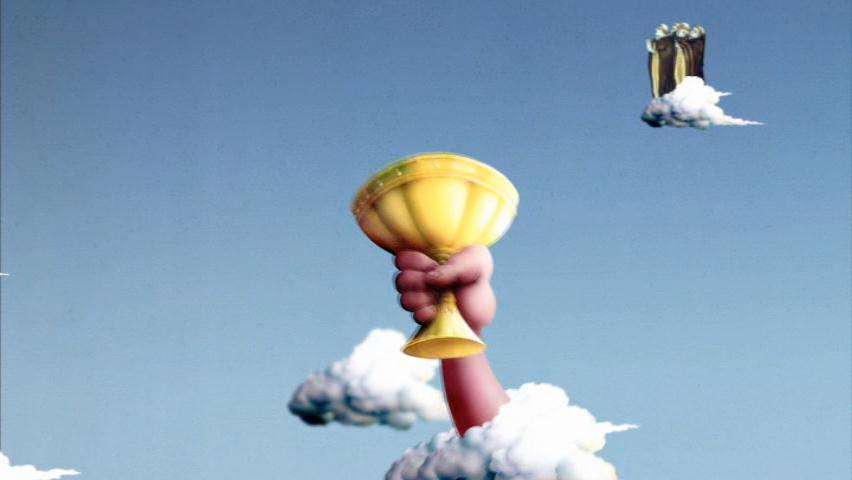
\includegraphics[width=0.8\textwidth]{grail.jpg}
%   \caption[Voorbeeld figuur.]{\label{fig:grail}Voorbeeld van invoegen van een figuur. Zorg altijd voor een uitgebreid bijschrift dat de figuur volledig beschrijft zonder in de tekst te moeten gaan zoeken. Vergeet ook je bronvermelding niet!}
% \end{figure}

% \begin{listing}
%   \begin{minted}{python}
%     import pandas as pd
%     import seaborn as sns

%     penguins = sns.load_dataset('penguins')
%     sns.relplot(data=penguins, x="flipper_length_mm", y="bill_length_mm", hue="species")
%   \end{minted}
%   \caption[Voorbeeld codefragment]{Voorbeeld van het invoegen van een codefragment.}
% \end{listing}

% \lipsum[7-20]

% \begin{table}
%   \centering
%   \begin{tabular}{lcr}
%     \toprule
%     \textbf{Kolom 1} & \textbf{Kolom 2} & \textbf{Kolom 3} \\
%     $\alpha$         & $\beta$          & $\gamma$         \\
%     \midrule
%     A                & 10.230           & a                \\
%     B                & 45.678           & b                \\
%     C                & 99.987           & c                \\
%     \bottomrule
%   \end{tabular}
%   \caption[Voorbeeld tabel]{\label{tab:example}Voorbeeld van een tabel.}
% \end{table}

%%=============================================================================
%% Methodologie
%%=============================================================================

\chapter{\IfLanguageName{dutch}{Methodologie}{Methodology}}%
\label{ch:methodologie}

The development process for this project is structured into distinct stages, each pursuing specific objectives, generating clear deliverables, and applying targeted research methods. The stages appear below.

\section{Tool Selection}
This stage selects a facial-recognition tool that balances accessibility, security and ease of integration.  
Following an extensive literature review and comparative analysis, the project adopts \textbf{face-api.js} based on:

\begin{itemize}
  \item \textbf{Privacy:} Face-api.js processes all data on the client, eliminating external transmission of biometric information and strengthening user privacy.
  \item \textbf{Compatibility:} The library integrates smoothly with modern 
  Java\-Script frameworks, streamlining development and reducing complexity.
  \item \textbf{Real-time performance:} Its lightweight, modular architecture enables efficient real-time operation—an essential feature for accessibility-centred web applications.
\end{itemize}

Alternatives such as \textbf{OpenCV (Java)} and \textbf{face\_recognition (Python)} are considered and benchmarked, yet face-api.js ultimately offers the best balance of performance, integration effort and suitability for client-side deployment.

\section{Prototype Development}
This phase develops a fully functional, web-based password manager that addresses usability and accessibility barriers for individuals with cognitive and motor disabilities. The prototype relies on TypeScript to maximise maintainability and robustness. Key deliverables in this stage include:

\begin{itemize}
  \item \textbf{Face-authentication module:} Users authenticate through facial recognition, removing the burden of remembering complex textual passwords.
  \item \textbf{Credential-management system:} Secure mechanisms store and retrieve user credentials.
  \item \textbf{Password-generation tool:} An integrated utility produces robust, unique passwords automatically.
  \item \textbf{Accessible user interface (UI):} The design follows Web Content Accessibility Guidelines (WCAG) to ensure usability—especially for users facing cognitive or motor challenges.
\end{itemize}

Development follows an iterative Agile methodology, enabling continuous refinement through intermediate testing and preliminary user feedback.

\section{Database Selection}
Choosing an efficient, secure database to manage user credentials forms a crucial component of the project. After evaluating multiple options against performance, security, scalability and integration criteria, the project currently employs:

\begin{itemize}
  \item \textbf{SQLite:} Adopted for the initial prototype because of its simplicity, lightweight footprint and suitability for local client-side storage.
  \item \textbf{PostgreSQL:} Evaluated for future scenarios that demand greater scalability, flexible data models and larger datasets.
\end{itemize}

Both database solutions undergo performance tests and security assessments during prototype development.

\section{Future Expansion and Scalability}
If the browser-based prototype proves successful, the next plan is to
package it as an \textbf{offline-first Chrome extension}.  
SQLite's embedded design keeps the entire password vault in a single file
bundled with the extension, so no external server is required—precisely why
SQLite was chosen.  This direction will let users install the password manager
instantly from the Chrome Web Store and keep their credentials local while
still benefiting from auto-fill and seamless updates.

Planned next steps include:
\begin{itemize}
  \item Adapting the current React/TypeScript codebase to Chrome Extension
        APIs (manifest v3) for secure content-script injection and
        background tasks.
  \item Implementing permission-scoped access to web pages for auto-fill
        while preserving privacy.
  \item Testing storage limits and performance of the SQLite WASM build in
        Chrome to ensure smooth operation on low-end devices.
  \item Exploring optional cloud backup and multi-device sync as opt-in
        features, keeping the default experience fully offline.
\end{itemize}


%% TODO: In dit hoofstuk geef je een korte toelichting over hoe je te werk bent
%% gegaan. Verdeel je onderzoek in grote fasen, en licht in elke fase toe wat
%% de doelstelling was, welke deliverables daar uit gekomen zijn, en welke
%% onderzoeksmethoden je daarbij toegepast hebt. Verantwoord waarom je
%% op deze manier te werk gegaan bent.
%% 
%% Voorbeelden van zulke fasen zijn: literatuurstudie, opstellen van een
%% requirements-analyse, opstellen long-list (bij vergelijkende studie),
%% selectie van geschikte tools (bij vergelijkende studie, "short-list"),
%% opzetten testopstelling/PoC, uitvoeren testen en verzamelen
%% van resultaten, analyse van resultaten, ...
%%
%% !!!!! LET OP !!!!!
%%
%% Het is uitdrukkelijk NIET de bedoeling dat je het grootste deel van de corpus
%% van je bachelorproef in dit hoofstuk verwerkt! Dit hoofdstuk is eerder een
%% kort overzicht van je plan van aanpak.
%%
%% Maak voor elke fase (behalve het literatuuronderzoek) een NIEUW HOOFDSTUK aan
%% en geef het een gepaste titel.

% \lipsum[21-25]



% Voeg hier je eigen hoofdstukken toe die de ``corpus'' van je bachelorproef
% vormen. De structuur en titels hangen af van je eigen onderzoek. Je kan bv.
% elke fase in je onderzoek in een apart hoofdstuk bespreken.

%% Implementatie
%%=============================================================================

\chapter{Prototype Implementation}%
\label{ch:implementatie}

% TODO: Add content for the implementation chapter here.
% This chapter should document the architecture of the web-based password manager.
% Cover the facial-authentication workflow, cryptographic handling of credentials
% with bcrypt, the WCAG-compliant user interface, and the modular codebase.

\section{Prototype Implementation}

\subsection{Architecture overview}
The password manager is implemented as a modern client-server web application.  
\begin{itemize}
  \item \textbf{Frontend} - a React single-page application (SPA) written in TypeScript delivers the user interface.  
  \item \textbf{Backend} - a Node.js\,/\,Express service, also in TypeScript, handles data persistence, face-recognition logic and JSON Web Token (JWT) issuance.  
  \item \textbf{Database} - user and credential data are stored in an SQLite file accessed through the Prisma ORM; a PostgreSQL target is available for future scaling.  
\end{itemize}

\subsection{Technology stack}
\paragraph{Frontend}
React {+} TypeScript, React Context API for state, Tailwind CSS components, Axios for REST calls, \texttt{crypto-js} for client-side AES-256 encryption, and \texttt{face-api.js} (TensorFlow.js) for in-browser face detection.

\paragraph{Backend}
Node.js 18, Express 4, TypeScript, Prisma, \texttt{face-api.js} running under \texttt{node-canvas} for server-side inference, JWT for session tokens, and the Node \texttt{crypto} module for cryptography.

\subsection{Face-authentication workflow}
\begin{enumerate}
  \item \textbf{Registration} - the browser captures a webcam frame, encrypts it with AES-256 under a user-specific key, and posts it to the server. After decryption, \texttt{face-api.js} extracts a 128-D descriptor that is stored with the user record.
  \item \textbf{Login} - a fresh frame is captured, encrypted and processed in the same way; its descriptor is compared to the stored vector with Euclidean distance~$\le0.6$. Our target threshold (FAR $\leq 0.1\%$, FRR $\leq 10\%$) is grounded in the industry figures summarised in Section~\ref{sec:biometric-benchmarks}.
  \item \textbf{Optimisation} - images are down-scaled (320\,$\times$\,240) and processed with TinyFaceDetector / MobileNet V1 models that are pre-loaded once at server start.
\end{enumerate}

\subsection{Secure credential vault}
\begin{itemize}
  \item Keys are derived client-side with PBKDF2 (10\,000 iterations, 16-byte salt).  
  \item All usernames and passwords are AES-256-CBC encrypted in the browser before transmission; only ciphertext is stored.  
  \item During retrieval the encrypted blobs are returned unchanged and decrypted locally, so plaintext secrets never leave the user's device.  
\end{itemize}

\subsection{Implementation roadmap}
Development progressed through the following incremental phases:

\begin{enumerate}[label=\textbf{Phase~\arabic*:}, leftmargin=2.5em]
  \item \emph{Requirements \& accessibility goals} - zero plaintext outside the browser and WCAG 2.2 AA compliance.%
  \item Dual-repo setup (\texttt{pwd-manager-frontend} \& \texttt{pwd-manager-backend}) merged into a monorepo with Nx, CI pipeline (ESLint, tests, Docker).%
  \item Core architecture: React + Vite SPA, Express API, Prisma models \emph{User} \& \emph{Credential}.%
  \item Face-authentication MVP using Tiny MobileNet V1 and in-browser matching.%
  \item End-to-end client-side cryptography (PBKDF2 $\rightarrow$ AES-256-CBC).%
  \item Credential-vault CRUD with optimistic UI updates and password-strength meter.%
  \item Transport security and DevOps: Nginx + Let's Encrypt, HSTS, CSP, multi-stage Docker images.%
  \item Accessibility pass and UI refinements.%
  \item Backup/restore via encrypted JSON and initial sync stubs for future cloud integration.%
  \item Quality assurance: Vitest, Jest, Playwright end-to-end tests, CI coverage $>$90\,\%.%
\end{enumerate}


\subsection{Database schema}
The \texttt{User} table stores the e-mail address and the 128-dimensional face descriptor; the \texttt{Credential} table stores website metadata together with encrypted username and password, and cascades on user deletion.


\subsection{Encryption and Decryption}\label{subsec:encryption}

All sensitive fields including passwords and webcam images are protected end-to-end with AES-256 encryption.
Keys are never transmitted in plaintext; instead they are derived client-side with PBKDF2 and reproduced server-side only when needed for decryption.

\subsubsection{Password encryption workflow}

\paragraph{Key derivation (PBKDF2).}
A 256-bit key is derived in the browser from a user-specific base key and a 16-byte salt, using 10000 iterations.

\begin{lstlisting}[language=TypeScript, caption={Key derivation function using PBKDF2}, label={lst:strengthen-key}]
export const strengthenKey = (baseKey: string): string => {
  return PBKDF2(baseKey, SALT, {
    keySize: KEY_SIZE / 32,   // 256 bits
    iterations: ITERATIONS,   // 10,000
  }).toString();
};
\end{lstlisting}

\paragraph{AES-256 encryption and decryption.}
The code below demonstrates the encryption and decryption functions used in the client. The encrypt function strengthens the provided key and uses AES to encrypt the value, while the decrypt function reverses this process with error handling.

\begin{lstlisting}[language=TypeScript, caption={AES-256 encryption and decryption functions}, label={lst:encrypt-decrypt}]
export const encrypt = (value: string, secretKey: string): string => {
  if (!value) return "";
  const strengthenedKey = strengthenKey(secretKey);
  return AES.encrypt(value, strengthenedKey).toString();
};

export const decrypt = (
  encryptedValue: string,
  secretKey: string
): string => {
  if (!encryptedValue) return "";
  try {
    const strengthenedKey = strengthenKey(secretKey);
    const bytes = AES.decrypt(encryptedValue, strengthenedKey);
    return bytes.toString(UTF8);
  } catch (error) {
    console.error("Failed to decrypt value:", error);
    return "";
  }
};
\end{lstlisting}

Each user obtains a unique secret based on their ID, e-mail and an application secret, as shown in the following function.

\begin{lstlisting}[language=TypeScript, caption={User-specific encryption key generation}, label={lst:user-key}]
export const getUserEncryptionKey = (
  userId: number,
  userEmail: string
): string => {
  const appSecretKey = import.meta.env.VITE_SECRET_KEY || "app-default-key";
  return `pwd-manager-${userId}-${userEmail}-${appSecretKey}`;
};
\end{lstlisting}

Before storage, credential fields are encrypted using the function below, which processes each sensitive field individually.

\begin{lstlisting}[language=TypeScript, caption={Encryption of credential fields before storage}, label={lst:encrypt-credential}]
const encryptCredential = (
  credential: CredentialEntry,
  encryptionKey: string
): EncryptedCredential => {
  return {
    ...credential,
    username: encrypt(credential.username, encryptionKey),
    password: encrypt(credential.password, encryptionKey),
    notes: credential.notes
      ? encrypt(credential.notes, encryptionKey)
      : undefined,
  };
};
\end{lstlisting}

\subsubsection{Face-image encryption workflow}

\paragraph{Client-side processing.}
A captured webcam frame is converted to Base64 and then encrypted with the same AES/PBKDF2 scheme, as demonstrated in the code below.

\begin{lstlisting}[language=TypeScript, caption={Client-side webcam image processing and encryption}, label={lst:image-processing}]
export const blobToBase64 = (blob: Blob): Promise<string> => {
  return new Promise((resolve, reject) => {
    const reader = new FileReader();
    reader.onloadend = () => {
      if (typeof reader.result === "string") {
        const base64 = reader.result.split(",")[1]; // strip data URL prefix
        resolve(base64);
      } else {
        reject(new Error("Failed to convert blob to base64"));
      }
    };
    reader.readAsDataURL(blob);
  });
};

export const encryptImage = async (
  imageBlob: Blob,
  encryptionKey: string
): Promise<{ encryptedData: string; contentType: string }> => {
  const base64Data = await blobToBase64(imageBlob);
  const encryptedData = encrypt(base64Data, encryptionKey);
  return { encryptedData, contentType: imageBlob.type };
};
\end{lstlisting}

Encrypted payloads are packaged into a `FormData` object for upload using the following utility function.

\begin{lstlisting}[language=TypeScript, caption={Creation of FormData for encrypted image upload}, label={lst:form-data}]
export const createEncryptedImageFormData = async (
  imageBlob: Blob,
  encryptionKey: string,
  fieldName: string = "image",
  additionalData: Record<string, string> = {}
): Promise<FormData> => {
  const { encryptedData, contentType } =
    await encryptImage(imageBlob, encryptionKey);

  const formData = new FormData();
  formData.append(`${fieldName}Encrypted`, encryptedData);
  formData.append(`${fieldName}ContentType`, contentType);
  formData.append(`${fieldName}IsEncrypted`, "true");
  Object.entries(additionalData).forEach(([k, v]) =>
    formData.append(k, v)
  );
  return formData;
};
\end{lstlisting}

\paragraph{Server-side decryption.}
The backend reproduces the key, then performs AES-256-CBC decryption as demonstrated in the server-side functions below.

\begin{lstlisting}[language=TypeScript, caption={Server-side decryption of encrypted data from the frontend}, label={lst:server-decryption}]
export const decryptFromFrontend = (
  cipherText: string,
  password: string
): Buffer => {
  const parts = cipherText.split(":");        // salt:iv:data
  const salt = Buffer.from(parts[0], "hex");
  const iv   = Buffer.from(parts[1], "hex");
  const encryptedData = Buffer.from(parts[2], "base64");

  const key = deriveKey(password, salt);      // PBKDF2
  const decipher = crypto.createDecipheriv(
    CRYPTO_CONFIG.algorithm, key, iv
  );
  return Buffer.concat([decipher.update(encryptedData), decipher.final()]);
};

export const decryptUserImage = (
  encryptedBase64: string,
  userId: number,
  userEmail: string
): Buffer => {
  const encryptionKey = getUserEncryptionKey(userId, userEmail);
  return decryptFromFrontend(encryptedBase64, encryptionKey);
};
\end{lstlisting}

\subsubsection{Security guarantees}

\begin{itemize}
  \item \textbf{End-to-end encryption}: passwords and images are encrypted in the browser; only ciphertext and face descriptors are stored.  
  \item \textbf{Per-user keys}: each key binds the user's ID and e-mail to an application secret, preventing key reuse across accounts.  
  \item \textbf{Key strengthening}: PBKDF2 with 10 000 iterations thwarts brute-force attacks on weak secrets.  
  \item \textbf{Compatible crypto}: frontend (\texttt{crypto-js}) and backend (\texttt{node:crypto}) use identical AES-256-CBC parameters, ensuring seamless decryption.  
\end{itemize}



%%=============================================================================
%% Conclusie
%%=============================================================================

\chapter{Discussion}%
\label{ch:conclusie}

% TODO: Trek een duidelijke conclusie, in de vorm van een antwoord op de
% onderzoeksvra(a)g(en). Wat was jouw bijdrage aan het onderzoeksdomein en
% hoe biedt dit meerwaarde aan het vakgebied/doelgroep? 
% Reflecteer kritisch over het resultaat. In Engelse teksten wordt deze sectie
% ``Discussion'' genoemd. Had je deze uitkomst verwacht? Zijn er zaken die nog
% niet duidelijk zijn?
% Heeft het onderzoek geleid tot nieuwe vragen die uitnodigen tot verder 
%onderzoek?

\lipsum[76-80]



%---------- Bijlagen -----------------------------------------------------------

\appendix

\chapter{Research Proposal}
The subject of this bachelor's thesis is based on a research proposal that was evaluated beforehand by the promotor. That proposal is included in this appendix.

%% TODO: 
%\section*{Samenvatting}

% Kopieer en plak hier de samenvatting (abstract) van je onderzoeksvoorstel.
    The increasing reliance on online services has elevated the importance of password management in digital security. Traditional authentication methods, such as typing and remembering complex passwords, often pose significant challenges for individuals with cognitive or motor disabilities, such as difficulties with memory recall or typing. These challenges highlight the need for accessible authentication solutions that enhance user satisfaction and experience. This proposal examines the potential of integrating face recognition technology as an accessible authentication mechanism in password management, specifically for individuals with cognitive and motor disabilities.
    The primary research question is: How can face recognition technology improve accessibility in password management for individuals with cognitive and motor disabilities? The research will involve analyzing various face recognition APIs across multiple programming languages to identify the most suitable technology and programming language for this use case. Based on the findings, a web-based prototype password manager will be developed using the chosen technologies. If successful, the next step will involve creating a desktop application to evaluate the scalability and effectiveness of the selected solutions. This iterative methodology ensures a well-informed and comprehensive evaluation of the technologies before full implementation.
    Expected outcomes include improved accessibility and usability compared to traditional password managers, leading to measurable enhancements in user satisfaction and reduced frustration during authentication processes. This study aims to demonstrate the potential of face recognition technology to address accessibility challenges in password management, helping individuals with cognitive and motor disabilities to independently and effectively manage their digital credentials.

% Verwijzing naar het bestand met de inhoud van het onderzoeksvoorstel
%---------- Inleiding ---------------------------------------------------------

% TODO: Is dit voorstel gebaseerd op een paper van Research Methods die je
% vorig jaar hebt ingediend? Heb je daarbij eventueel samengewerkt met een
% andere student?
% Zo ja, haal dan de tekst hieronder uit commentaar en pas aan.

%\paragraph{Opmerking}

% Dit voorstel is gebaseerd op het onderzoeksvoorstel dat werd geschreven in het
% kader van het vak Research Methods dat ik (vorig/dit) academiejaar heb
% uitgewerkt (met medesturent VOORNAAM NAAM als mede-auteur).
% 

\section{Inleiding}%
\label{sec:inleiding}

Waarover zal je bachelorproef gaan? Introduceer het thema en zorg dat volgende zaken zeker duidelijk aanwezig zijn:

\begin{itemize}
  \item kaderen thema
  \item de doelgroep
  \item de probleemstelling en (centrale) onderzoeksvraag
  \item de onderzoeksdoelstelling
\end{itemize}

Denk er aan: een typische bachelorproef is \textit{toegepast onderzoek}, wat betekent dat je start vanuit een concrete probleemsituatie in bedrijfscontext, een \textbf{casus}. Het is belangrijk om je onderwerp goed af te bakenen: je gaat voor die \textit{ene specifieke probleemsituatie} op zoek naar een goede oplossing, op basis van de huidige kennis in het vakgebied.

De doelgroep moet ook concreet en duidelijk zijn, dus geen algemene of vaag gedefinieerde groepen zoals \emph{bedrijven}, \emph{developers}, \emph{Vlamingen}, enz. Je richt je in elk geval op it-professionals, een bachelorproef is geen populariserende tekst. Eén specifiek bedrijf (die te maken hebben met een concrete probleemsituatie) is dus beter dan \emph{bedrijven} in het algemeen.

Formuleer duidelijk de onderzoeksvraag! De begeleiders lezen nog steeds te veel voorstellen waarin we geen onderzoeksvraag terugvinden.

Schrijf ook iets over de doelstelling. Wat zie je als het concrete eindresultaat van je onderzoek, naast de uitgeschreven scriptie? Is het een proof-of-concept, een rapport met aanbevelingen, \ldots Met welk eindresultaat kan je je bachelorproef als een succes beschouwen?

%---------- Stand van zaken ---------------------------------------------------

\section{Literatuurstudie}%
\label{sec:literatuurstudie}

Hier beschrijf je de \emph{state-of-the-art} rondom je gekozen onderzoeksdomein, d.w.z.\ een inleidende, doorlopende tekst over het onderzoeksdomein van je bachelorproef. Je steunt daarbij heel sterk op de professionele \emph{vakliteratuur}, en niet zozeer op populariserende teksten voor een breed publiek. Wat is de huidige stand van zaken in dit domein, en wat zijn nog eventuele open vragen (die misschien de aanleiding waren tot je onderzoeksvraag!)?

Je mag de titel van deze sectie ook aanpassen (literatuurstudie, stand van zaken, enz.). Zijn er al gelijkaardige onderzoeken gevoerd? Wat concluderen ze? Wat is het verschil met jouw onderzoek?

Verwijs bij elke introductie van een term of bewering over het domein naar de vakliteratuur, bijvoorbeeld~\autocite{Hykes2013}! Denk zeker goed na welke werken je refereert en waarom.

Draag zorg voor correcte literatuurverwijzingen! Een bronvermelding hoort thuis \emph{binnen} de zin waar je je op die bron baseert, dus niet er buiten! Maak meteen een verwijzing als je gebruik maakt van een bron. Doe dit dus \emph{niet} aan het einde van een lange paragraaf. Baseer nooit teveel aansluitende tekst op eenzelfde bron.

Als je informatie over bronnen verzamelt in JabRef, zorg er dan voor dat alle nodige info aanwezig is om de bron terug te vinden (zoals uitvoerig besproken in de lessen Research Methods).

% Voor literatuurverwijzingen zijn er twee belangrijke commando's:
% \autocite{KEY} => (Auteur, jaartal) Gebruik dit als de naam van de auteur
%   geen onderdeel is van de zin.
% \textcite{KEY} => Auteur (jaartal)  Gebruik dit als de auteursnaam wel een
%   functie heeft in de zin (bv. ``Uit onderzoek door Doll & Hill (1954) bleek
%   ...'')

Je mag deze sectie nog verder onderverdelen in subsecties als dit de structuur van de tekst kan verduidelijken.

%---------- Methodologie ------------------------------------------------------
\section{Methodologie}%
\label{sec:methodologie}

Hier beschrijf je hoe je van plan bent het onderzoek te voeren. Welke onderzoekstechniek ga je toepassen om elk van je onderzoeksvragen te beantwoorden? Gebruik je hiervoor literatuurstudie, interviews met belanghebbenden (bv.~voor requirements-analyse), experimenten, simulaties, vergelijkende studie, risico-analyse, PoC, \ldots?

Valt je onderwerp onder één van de typische soorten bachelorproeven die besproken zijn in de lessen Research Methods (bv.\ vergelijkende studie of risico-analyse)? Zorg er dan ook voor dat we duidelijk de verschillende stappen terug vinden die we verwachten in dit soort onderzoek!

Vermijd onderzoekstechnieken die geen objectieve, meetbare resultaten kunnen opleveren. Enquêtes, bijvoorbeeld, zijn voor een bachelorproef informatica meestal \textbf{niet geschikt}. De antwoorden zijn eerder meningen dan feiten en in de praktijk blijkt het ook bijzonder moeilijk om voldoende respondenten te vinden. Studenten die een enquête willen voeren, hebben meestal ook geen goede definitie van de populatie, waardoor ook niet kan aangetoond worden dat eventuele resultaten representatief zijn.

Uit dit onderdeel moet duidelijk naar voor komen dat je bachelorproef ook technisch voldoen\-de diepgang zal bevatten. Het zou niet kloppen als een bachelorproef informatica ook door bv.\ een student marketing zou kunnen uitgevoerd worden.

Je beschrijft ook al welke tools (hardware, software, diensten, \ldots) je denkt hiervoor te gebruiken of te ontwikkelen.

Probeer ook een tijdschatting te maken. Hoe lang zal je met elke fase van je onderzoek bezig zijn en wat zijn de concrete \emph{deliverables} in elke fase?

%---------- Verwachte resultaten ----------------------------------------------
\section{Verwacht resultaat, conclusie}%
\label{sec:verwachte_resultaten}

Hier beschrijf je welke resultaten je verwacht. Als je metingen en simulaties uitvoert, kan je hier al mock-ups maken van de grafieken samen met de verwachte conclusies. Benoem zeker al je assen en de onderdelen van de grafiek die je gaat gebruiken. Dit zorgt ervoor dat je concreet weet welk soort data je moet verzamelen en hoe je die moet meten.

Wat heeft de doelgroep van je onderzoek aan het resultaat? Op welke manier zorgt jouw bachelorproef voor een meerwaarde?

Hier beschrijf je wat je verwacht uit je onderzoek, met de motivatie waarom. Het is \textbf{niet} erg indien uit je onderzoek andere resultaten en conclusies vloeien dan dat je hier beschrijft: het is dan juist interessant om te onderzoeken waarom jouw hypothesen niet overeenkomen met de resultaten.



%%---------- Andere bijlagen --------------------------------------------------
% TODO: Voeg hier eventuele andere bijlagen toe. Bv. als je deze BP voor de
% tweede keer indient, een overzicht van de verbeteringen t.o.v. het origineel.
%\input{...}

%%---------- Backmatter, referentielijst ---------------------------------------

\backmatter{}

\setlength\bibitemsep{2pt} %% Add Some space between the bibliograpy entries
\printbibliography[heading=bibintoc]

\end{document}
